% Options for packages loaded elsewhere
\PassOptionsToPackage{unicode}{hyperref}
\PassOptionsToPackage{hyphens}{url}
\PassOptionsToPackage{dvipsnames,svgnames,x11names}{xcolor}
%
\documentclass[
  letterpaper,
  DIV=11,
  numbers=noendperiod]{scrartcl}

\usepackage{amsmath,amssymb}
\usepackage{iftex}
\ifPDFTeX
  \usepackage[T1]{fontenc}
  \usepackage[utf8]{inputenc}
  \usepackage{textcomp} % provide euro and other symbols
\else % if luatex or xetex
  \usepackage{unicode-math}
  \defaultfontfeatures{Scale=MatchLowercase}
  \defaultfontfeatures[\rmfamily]{Ligatures=TeX,Scale=1}
\fi
\usepackage{lmodern}
\ifPDFTeX\else  
    % xetex/luatex font selection
\fi
% Use upquote if available, for straight quotes in verbatim environments
\IfFileExists{upquote.sty}{\usepackage{upquote}}{}
\IfFileExists{microtype.sty}{% use microtype if available
  \usepackage[]{microtype}
  \UseMicrotypeSet[protrusion]{basicmath} % disable protrusion for tt fonts
}{}
\makeatletter
\@ifundefined{KOMAClassName}{% if non-KOMA class
  \IfFileExists{parskip.sty}{%
    \usepackage{parskip}
  }{% else
    \setlength{\parindent}{0pt}
    \setlength{\parskip}{6pt plus 2pt minus 1pt}}
}{% if KOMA class
  \KOMAoptions{parskip=half}}
\makeatother
\usepackage{xcolor}
\setlength{\emergencystretch}{3em} % prevent overfull lines
\setcounter{secnumdepth}{-\maxdimen} % remove section numbering
% Make \paragraph and \subparagraph free-standing
\makeatletter
\ifx\paragraph\undefined\else
  \let\oldparagraph\paragraph
  \renewcommand{\paragraph}{
    \@ifstar
      \xxxParagraphStar
      \xxxParagraphNoStar
  }
  \newcommand{\xxxParagraphStar}[1]{\oldparagraph*{#1}\mbox{}}
  \newcommand{\xxxParagraphNoStar}[1]{\oldparagraph{#1}\mbox{}}
\fi
\ifx\subparagraph\undefined\else
  \let\oldsubparagraph\subparagraph
  \renewcommand{\subparagraph}{
    \@ifstar
      \xxxSubParagraphStar
      \xxxSubParagraphNoStar
  }
  \newcommand{\xxxSubParagraphStar}[1]{\oldsubparagraph*{#1}\mbox{}}
  \newcommand{\xxxSubParagraphNoStar}[1]{\oldsubparagraph{#1}\mbox{}}
\fi
\makeatother


\providecommand{\tightlist}{%
  \setlength{\itemsep}{0pt}\setlength{\parskip}{0pt}}\usepackage{longtable,booktabs,array}
\usepackage{calc} % for calculating minipage widths
% Correct order of tables after \paragraph or \subparagraph
\usepackage{etoolbox}
\makeatletter
\patchcmd\longtable{\par}{\if@noskipsec\mbox{}\fi\par}{}{}
\makeatother
% Allow footnotes in longtable head/foot
\IfFileExists{footnotehyper.sty}{\usepackage{footnotehyper}}{\usepackage{footnote}}
\makesavenoteenv{longtable}
\usepackage{graphicx}
\makeatletter
\def\maxwidth{\ifdim\Gin@nat@width>\linewidth\linewidth\else\Gin@nat@width\fi}
\def\maxheight{\ifdim\Gin@nat@height>\textheight\textheight\else\Gin@nat@height\fi}
\makeatother
% Scale images if necessary, so that they will not overflow the page
% margins by default, and it is still possible to overwrite the defaults
% using explicit options in \includegraphics[width, height, ...]{}
\setkeys{Gin}{width=\maxwidth,height=\maxheight,keepaspectratio}
% Set default figure placement to htbp
\makeatletter
\def\fps@figure{htbp}
\makeatother

\KOMAoption{captions}{tableheading}
\makeatletter
\@ifpackageloaded{caption}{}{\usepackage{caption}}
\AtBeginDocument{%
\ifdefined\contentsname
  \renewcommand*\contentsname{Table of contents}
\else
  \newcommand\contentsname{Table of contents}
\fi
\ifdefined\listfigurename
  \renewcommand*\listfigurename{List of Figures}
\else
  \newcommand\listfigurename{List of Figures}
\fi
\ifdefined\listtablename
  \renewcommand*\listtablename{List of Tables}
\else
  \newcommand\listtablename{List of Tables}
\fi
\ifdefined\figurename
  \renewcommand*\figurename{Figure}
\else
  \newcommand\figurename{Figure}
\fi
\ifdefined\tablename
  \renewcommand*\tablename{Table}
\else
  \newcommand\tablename{Table}
\fi
}
\@ifpackageloaded{float}{}{\usepackage{float}}
\floatstyle{ruled}
\@ifundefined{c@chapter}{\newfloat{codelisting}{h}{lop}}{\newfloat{codelisting}{h}{lop}[chapter]}
\floatname{codelisting}{Listing}
\newcommand*\listoflistings{\listof{codelisting}{List of Listings}}
\makeatother
\makeatletter
\makeatother
\makeatletter
\@ifpackageloaded{caption}{}{\usepackage{caption}}
\@ifpackageloaded{subcaption}{}{\usepackage{subcaption}}
\makeatother

\ifLuaTeX
  \usepackage{selnolig}  % disable illegal ligatures
\fi
\usepackage{bookmark}

\IfFileExists{xurl.sty}{\usepackage{xurl}}{} % add URL line breaks if available
\urlstyle{same} % disable monospaced font for URLs
\hypersetup{
  pdftitle={Mortality Descriptives},
  colorlinks=true,
  linkcolor={blue},
  filecolor={Maroon},
  citecolor={Blue},
  urlcolor={Blue},
  pdfcreator={LaTeX via pandoc}}


\title{Mortality Descriptives}
\author{}
\date{}

\begin{document}
\maketitle


\subsection{Descriptive Statistics}\label{descriptive-statistics}

The following document is an exploratory data analysis of global data
from the World Bank describing conflict related mortality (i.e.,
maternal, neonate, under-5, and Infant mortality) between the years
2000-2019.

\subsection{There are 186 countries represented in this
data}\label{there-are-186-countries-represented-in-this-data}

The following table shows the countries with the greatest number of
annual conflicts between 2000-2019\ldots{}

\begin{longtable}[]{@{}lr@{}}
\caption{Top 25 countries with the highest number of
conflicts}\tabularnewline
\toprule\noalign{}
ISO & conflict\_count \\
\midrule\noalign{}
\endfirsthead
\toprule\noalign{}
ISO & conflict\_count \\
\midrule\noalign{}
\endhead
\bottomrule\noalign{}
\endlastfoot
AFG & 20 \\
COD & 20 \\
COL & 20 \\
DZA & 20 \\
ETH & 20 \\
IND & 20 \\
IRQ & 20 \\
MMR & 20 \\
NGA & 20 \\
PAK & 20 \\
PHL & 20 \\
RUS & 20 \\
SDN & 20 \\
SOM & 20 \\
KEN & 18 \\
TUR & 18 \\
THA & 17 \\
MEX & 16 \\
BDI & 15 \\
TCD & 15 \\
VEN & 15 \\
BRA & 14 \\
CAF & 14 \\
IRN & 13 \\
UGA & 13 \\
\end{longtable}

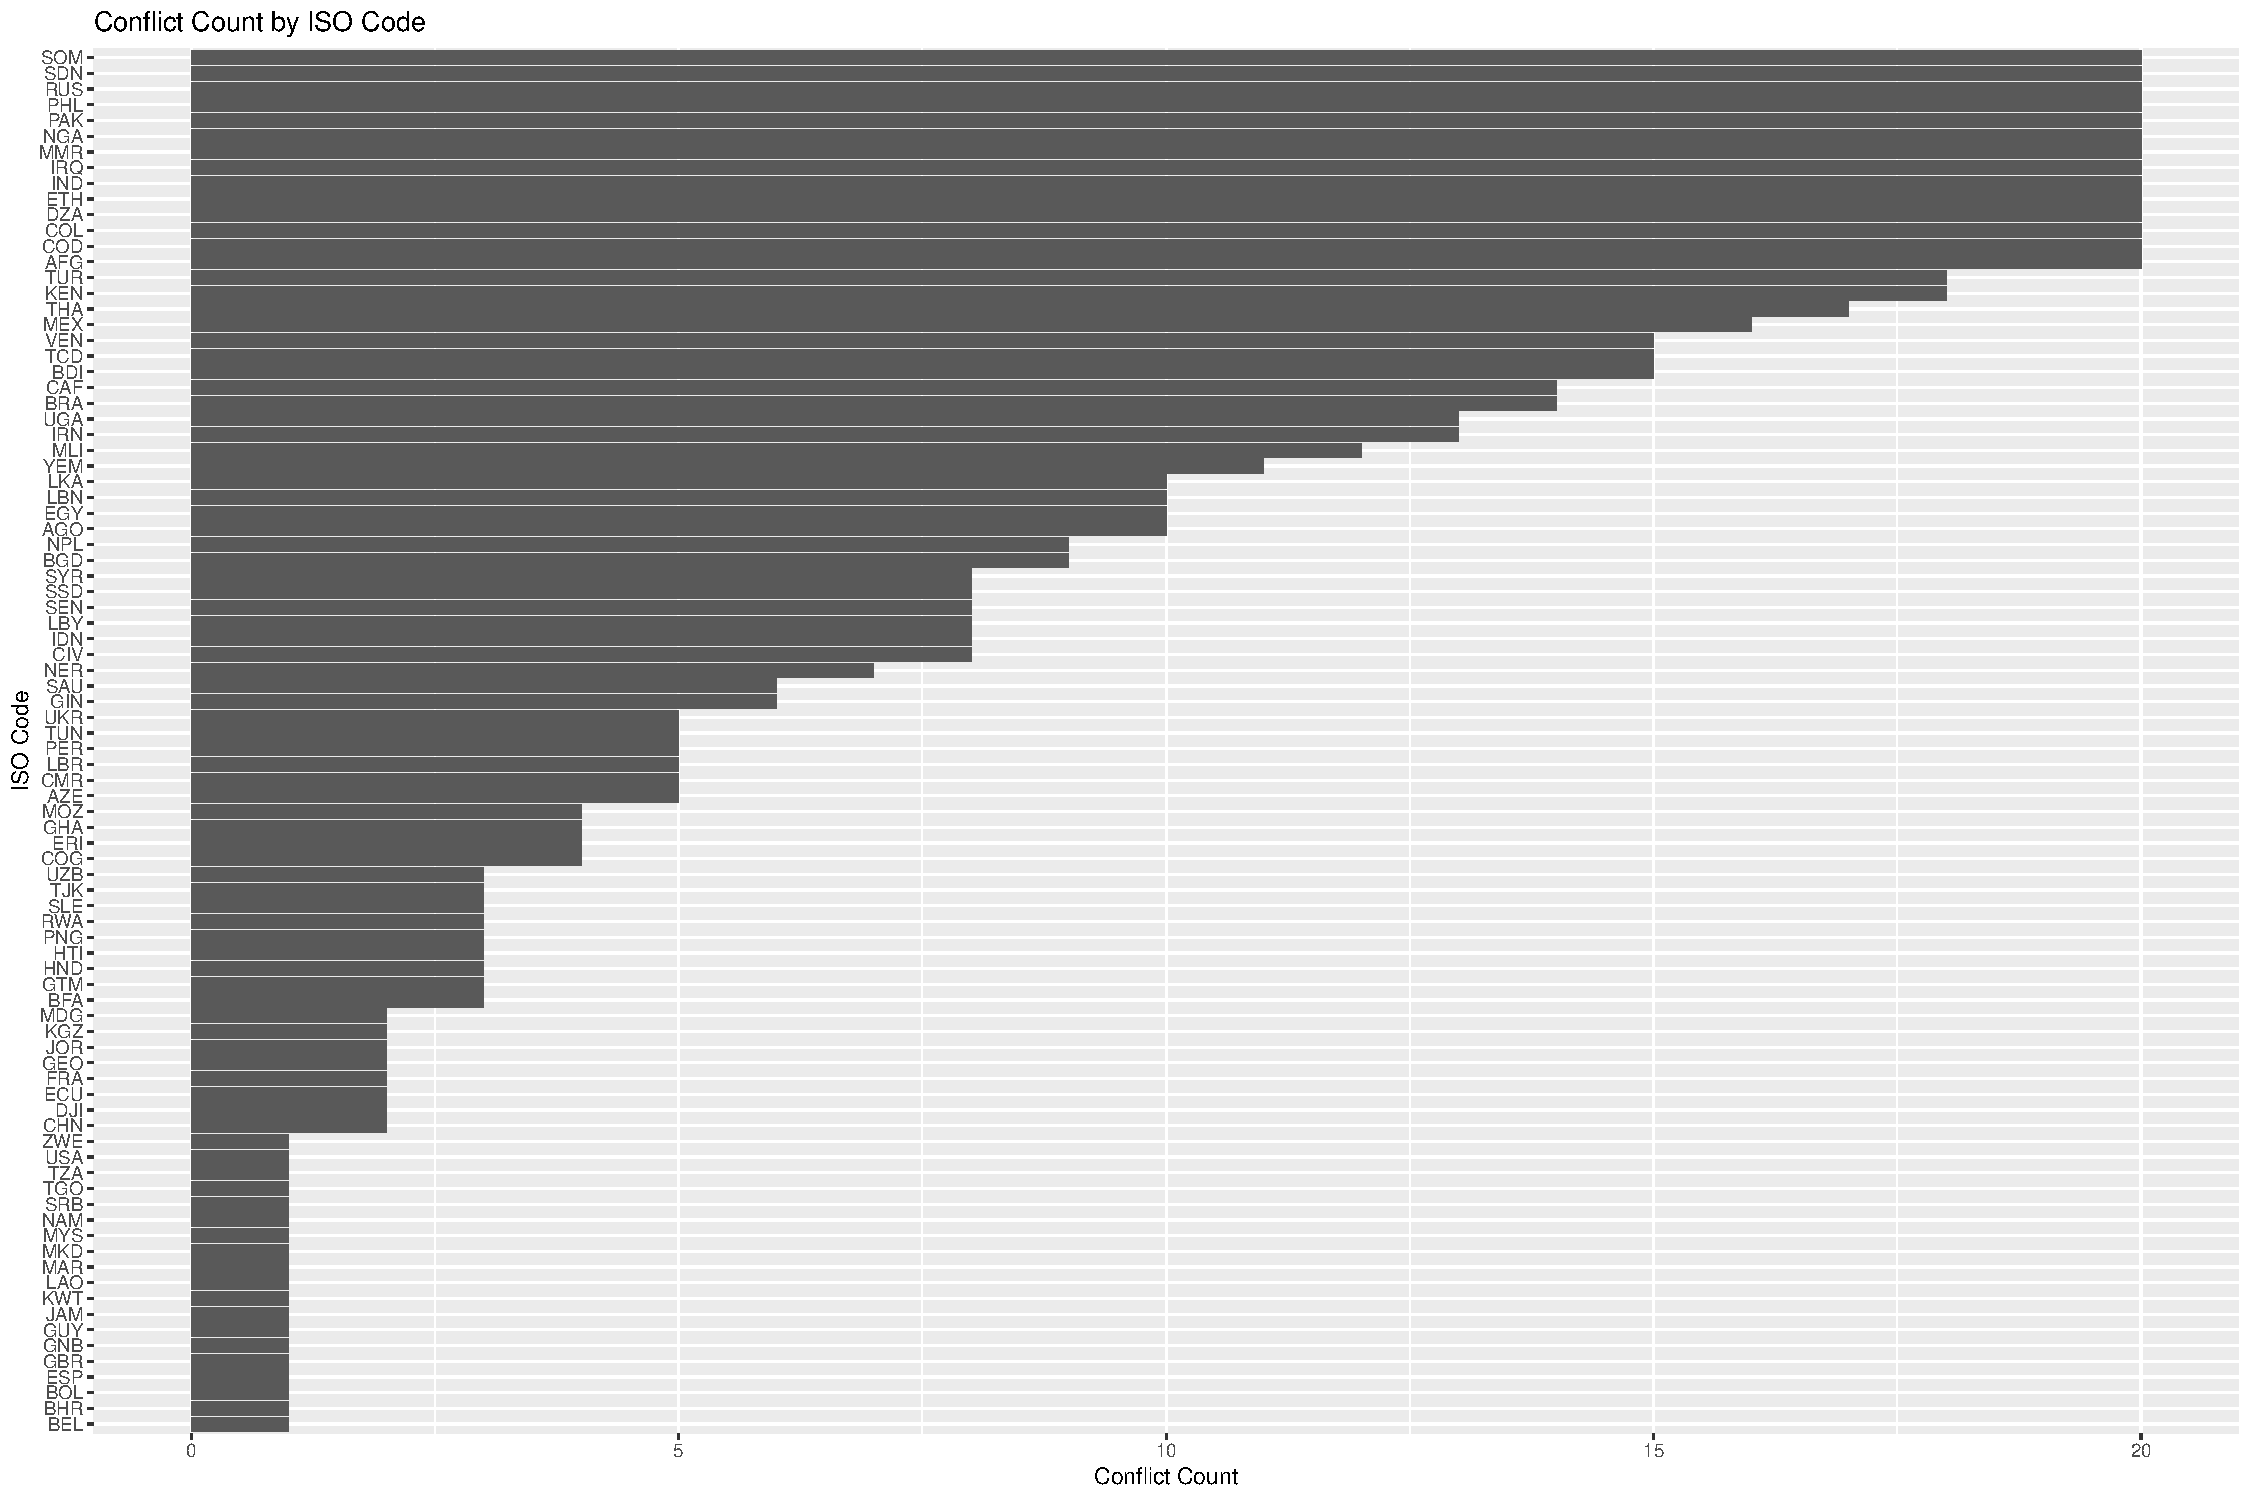
\includegraphics{MortalityDescriptives_files/figure-pdf/unnamed-chunk-3-1.pdf}

\subsection{Now, let us observe the total number of conflict related
deaths for each country between
2000-2019\ldots{}}\label{now-let-us-observe-the-total-number-of-conflict-related-deaths-for-each-country-between-2000-2019}

\begin{longtable}[]{@{}lr@{}}
\caption{Top 25 countries with the highest number of conflict related
deaths}\tabularnewline
\toprule\noalign{}
ISO & total\_best\_sum \\
\midrule\noalign{}
\endfirsthead
\toprule\noalign{}
ISO & total\_best\_sum \\
\midrule\noalign{}
\endhead
\bottomrule\noalign{}
\endlastfoot
SYR & 386891 \\
AFG & 171391 \\
IRQ & 91429 \\
ETH & 87066 \\
COD & 52492 \\
SDN & 51355 \\
NGA & 51114 \\
PAK & 40789 \\
IND & 32704 \\
MEX & 32686 \\
LKA & 29559 \\
SOM & 28049 \\
YEM & 26234 \\
COL & 23339 \\
RUS & 19322 \\
ERI & 19078 \\
PHL & 13660 \\
CAF & 12299 \\
NPL & 11854 \\
LBY & 11498 \\
SSD & 11304 \\
MMR & 10405 \\
BDI & 9281 \\
UGA & 9038 \\
DZA & 8648 \\
\end{longtable}

\subsection{The top 3 countries with the highest number of conflict
related deaths between 2000-2019 are
:}\label{the-top-3-countries-with-the-highest-number-of-conflict-related-deaths-between-2000-2019-are}

\begin{enumerate}
\def\labelenumi{\arabic{enumi}.}
\item
  \textbf{Syria}
\item
  \textbf{Afghanistan}
\item
  \textbf{Iraq}
\end{enumerate}

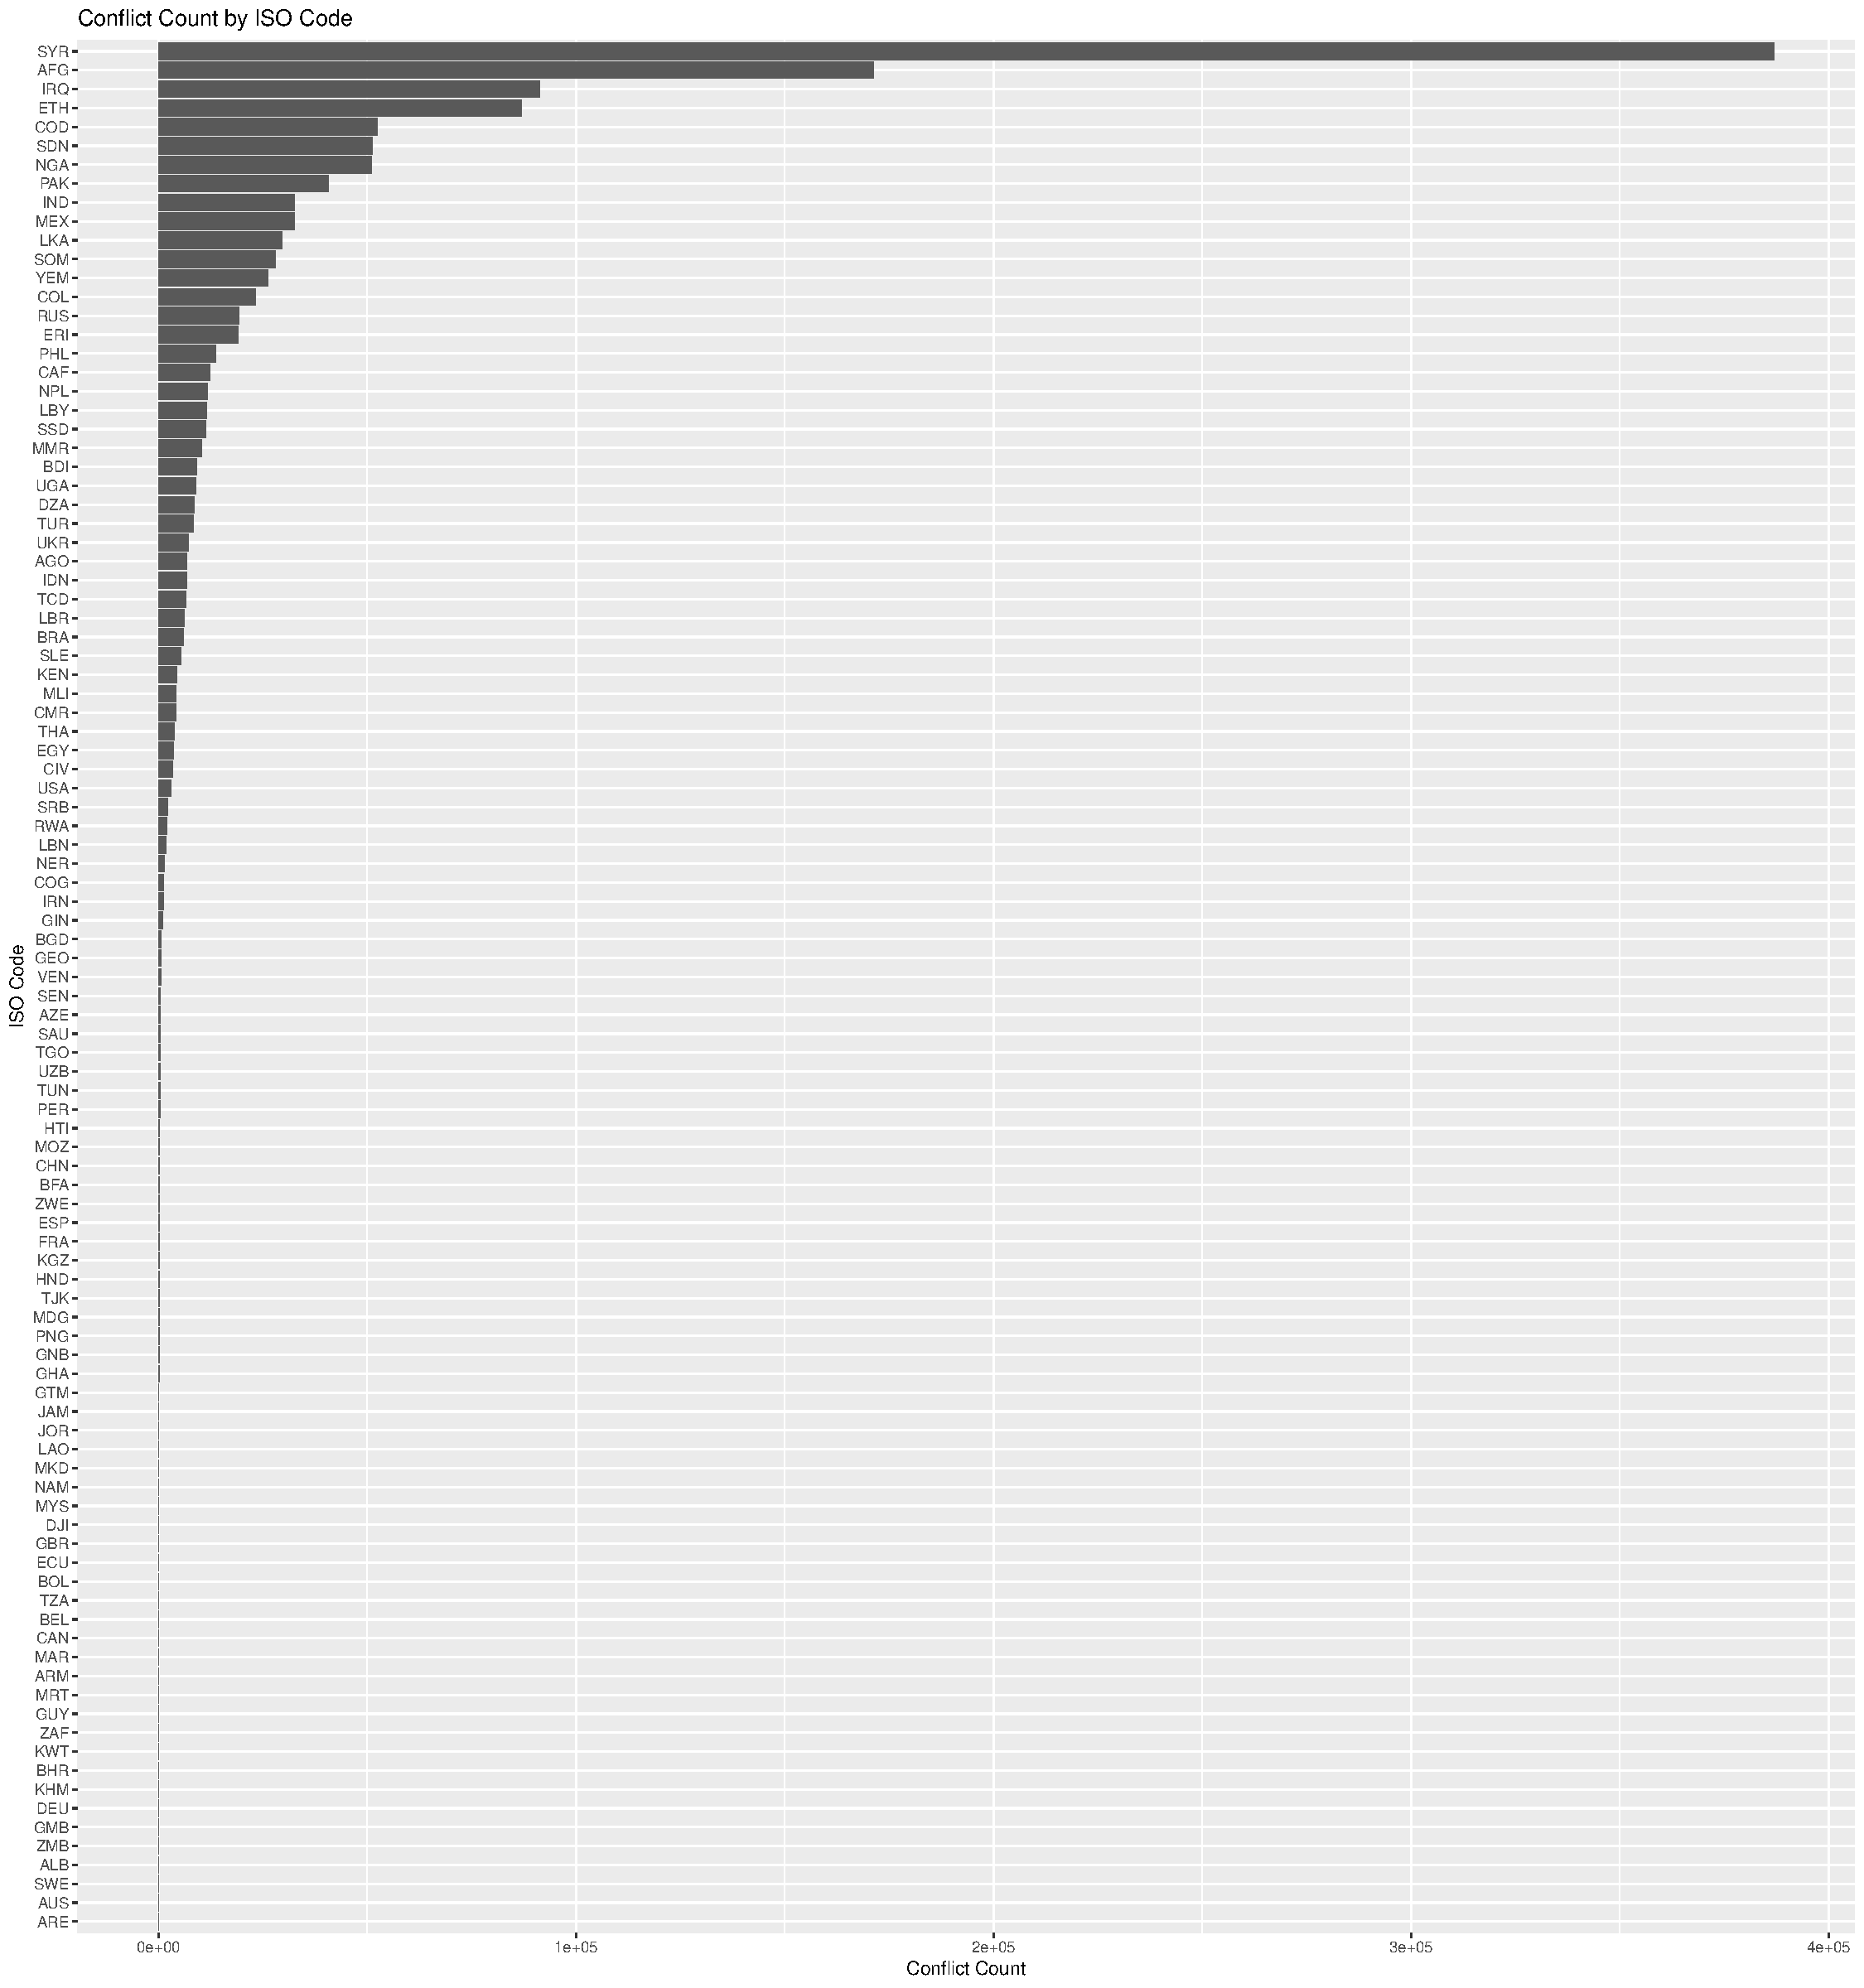
\includegraphics{MortalityDescriptives_files/figure-pdf/unnamed-chunk-5-1.pdf}

\subsubsection{In total there were 1343366 conflict-related deaths
between 2000-2019\ldots{} Before we analyze other trends, it will be
worth it to analyze our data structure and missingness
trends}\label{in-total-there-were-1343366-conflict-related-deaths-between-2000-2019-before-we-analyze-other-trends-it-will-be-worth-it-to-analyze-our-data-structure-and-missingness-trends}

\textbf{In total there are 21 variables in our dataset with the
following structure:}

\begin{itemize}
\item
  Character: country\_name, iSO, region
\item
  Integer: year, OECD, OECD2023, Matmor, conflict\_flag, drought,
  earthquake
\item
  Numeric: gdp1000, popdens, urban, agedep, male\_edu, temp,
  rainfall1000, InfMor, NeoMor, Under5Mor
\end{itemize}

\subsection{Let's check the missingness for all our variables and
identify the type of
missingness}\label{lets-check-the-missingness-for-all-our-variables-and-identify-the-type-of-missingness}

Let us determine which type of missing data we have in this
dataset\ldots{}

\begin{verbatim}
# A tibble: 1 x 4
  statistic    df p.value missing.patterns
      <dbl> <dbl>   <dbl>            <int>
1     1597.   125       0                8
\end{verbatim}

According to this Missing Completely At Random test, there is sufficient
evidence at the 5\% level to suggest that our data is not MCAR. This
means that our data is either missing at random or missing not at
random. Let us take a closer look\ldots{}

It is apparent from the plot above that missingness is not a significant
concern in our dataset with approximately \textbf{87\%} not having any
missing data across any of the 21 variables. Maternal mortality seems to
have the highest level of missingness (413 observations, 12.9\%).

From this plot, it is evident that some countries have complete
missingness observations for maternal mortality. These countries
include:

\begin{itemize}
\item
  ALB: Albania
\item
  CIV: Côte d'Ivoire (Ivory Coast)
\item
  MHL: Marshall Islands
\end{itemize}

It may be worthwhile to look at the connectedness of missingness across
various variables\ldots{}

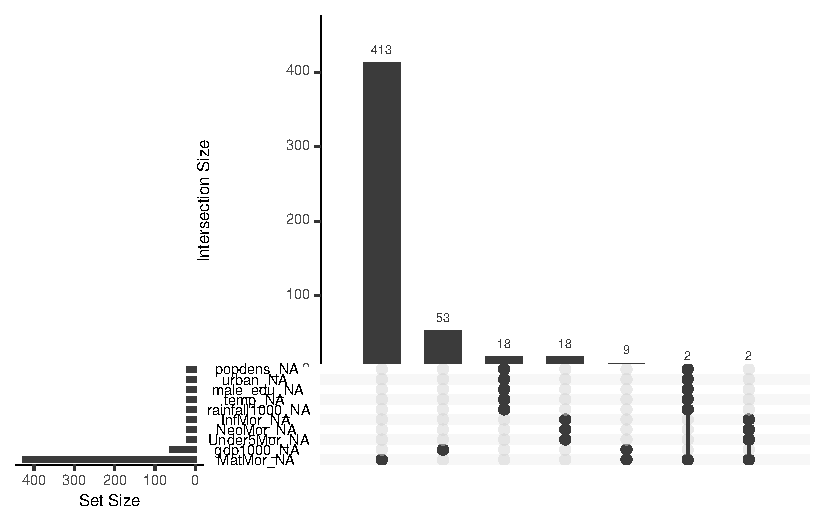
\includegraphics{MortalityDescriptives_files/figure-pdf/unnamed-chunk-11-1.pdf}

There seems to be two unique trends in missing values across
variables--- each of which show 18 separate observations of these two
trends!

\begin{enumerate}
\def\labelenumi{\arabic{enumi}.}
\tightlist
\item
  Urban, male\_edu, temp, rainfall1000
\item
  Infant mortality, neonatal mortality, and under-5 mortality.
\end{enumerate}

\section{Looking at variable specific
trends:}\label{looking-at-variable-specific-trends}

Summarizing the number of conflicts and deaths by region:

\begin{longtable}[]{@{}lr@{}}
\caption{Regions with the greatest number of conflict related
deaths}\tabularnewline
\toprule\noalign{}
region & total\_region \\
\midrule\noalign{}
\endfirsthead
\toprule\noalign{}
region & total\_region \\
\midrule\noalign{}
\endhead
\bottomrule\noalign{}
\endlastfoot
Western Asia & 516770 \\
Sub-Saharan Africa & 329930 \\
Southern Asia & 288238 \\
Northern Africa & 75563 \\
Latin America and the Caribbean & 64156 \\
South-eastern Asia & 34948 \\
Eastern Europe & 26489 \\
Northern America & 3045 \\
Southern Europe & 2514 \\
Central Asia & 851 \\
Eastern Asia & 299 \\
Western Europe & 291 \\
Melanesia & 202 \\
Northern Europe & 68 \\
Australia and New Zealand & 2 \\
Micronesia & 0 \\
Polynesia & 0 \\
\end{longtable}

It is apparent that African regions have the greatest conflict
attributed mortality in the world. Does the same trend occur with the
number of conflicts observed between 2000-2019?

\begin{longtable}[]{@{}lr@{}}
\caption{Regions with the greatest number of conflicts in the
world}\tabularnewline
\toprule\noalign{}
region & total\_cregion \\
\midrule\noalign{}
\endfirsthead
\toprule\noalign{}
region & total\_cregion \\
\midrule\noalign{}
\endhead
\bottomrule\noalign{}
\endlastfoot
Sub-Saharan Africa & 258 \\
Southern Asia & 101 \\
Latin America and the Caribbean & 84 \\
Western Asia & 84 \\
South-eastern Asia & 67 \\
Northern Africa & 64 \\
Eastern Europe & 25 \\
Central Asia & 8 \\
Melanesia & 3 \\
Southern Europe & 3 \\
Western Europe & 3 \\
Eastern Asia & 2 \\
Northern America & 1 \\
Northern Europe & 1 \\
Australia and New Zealand & 0 \\
Micronesia & 0 \\
Polynesia & 0 \\
\end{longtable}

\subsubsection{Let's take a look at more specific types of mortality and
relationships of other
variables\ldots{}}\label{lets-take-a-look-at-more-specific-types-of-mortality-and-relationships-of-other-variables}

\begin{longtable}[]{@{}lr@{}}
\caption{Countries with the greatest most number of
droughts}\tabularnewline
\toprule\noalign{}
ISO & total\_dISO \\
\midrule\noalign{}
\endfirsthead
\toprule\noalign{}
ISO & total\_dISO \\
\midrule\noalign{}
\endhead
\bottomrule\noalign{}
\endlastfoot
CHN & 14 \\
THA & 9 \\
USA & 9 \\
BRA & 8 \\
HND & 8 \\
KEN & 8 \\
SOM & 8 \\
BOL & 7 \\
ETH & 7 \\
MDG & 7 \\
MOZ & 7 \\
NER & 6 \\
PRY & 6 \\
AFG & 5 \\
BDI & 5 \\
GTM & 5 \\
IND & 5 \\
\end{longtable}




\end{document}
